\subsection{Previous Methods.}

We method produces a word distribution for teach test document and
outputs the most frequently unseen words in this distribution.

\begin{itemize}

\item
{\bf Baseline:} uses the training set word distribution. 

\item
{\bf KNN:} KNN finds the $k$ most similar training documents to a
testing document, where similarity is defined as the cosine between
the two documents as vectors in the word space. For a testing
document, KNN predicts the $s$ unseen words that are most frequent in
its $k$ closest training documents. Notice baseline is just KNN with
$k$ equal to the number of training documents.


\item
{\bf LDA:} Davide Blei's implementation \cite{LDAcode} based of
variational EM uses an ``estimation'' phase to train a topic model on
the training data.  Then use the ``inference'' routine to infer a
topic distribution for a test document which than uses the topic
definitions to produce a word distribution for the document.

\item
{K-means:} Uses $k$-means with cosine similaritly to produce
a topic matrix, and uses LDA inference to produce a word
distibution for each test document. 

\item
{\bf LDA(MALLET)} Uses the implementation of LDA in Mallet
based on Gibbs sampling \cite{McCallumMALLET}

\item {\bf LDAT, LDAC} For generated LDA datasets, we have two
  "cheating" algorithms as benchmarks. LDAT knows the real term-topic
  matrix $A$ of the model and uses the ``inference'' routine to find a
  word distribution for each document.  LDAC knows the real
  term-document matrix $M$ for each testing document, and uses the
  real word distribution for a test document.  LDAC is the best we can
  do given sampling noise.

\item {\bf LSI}.  Computes the best rank $k$ subspace approximation of the document-word
matrix.  Then projects test document into the subspace to find a word distribution.

\item {\bf Projector}. We have two versions of Projector which
is described below which produces a topic word matrix.  Then
LDA inference is used on each test document to produce
a word distribution. 

\end{itemize}

%% \subsection{LSI}
%% In the LDA model, we have $M=AW$, where $A$ and $W$ are the word-topic matrix and topic-document matrix respectively. Each column of M is a probability distribution on words. The $i$th document we observe is a set of i.i.d samples from the distribution $M_i$, and we have the observed word distribution $\hat{M}_i$. In the word space $\mathbb{R}^m$, all colunms of $M$ lie in the $k$-dimensional subspace spanned by the $k$ topics $A$. The sampled document $\hat{M}_i$ will be a noisy version of $M_i$, so in the word space $\mathbb{R}^m$, the points in $\hat{M}$ will be scattered close to the subspace of $A$.

%% LSI works by computing the best rank $k$ approximation to $\hat{M}$ of the training documents
%% \begin{align*}
%% &min_{U,\Sigma,V}\norm{\hat{M}-U\Sigma V}_F\\
%% \text{such that } &U\in \mathbb{R}^{m\times k},V\in \mathbb{R}^{k\times n}\text{  } orthonormal, \Sigma\in \mathbb{R}^{k\times k}\text{ }diagonal.
%% \end{align*}
%% The optimal $U,S,V$ are computed using singular value decomposition
%% (SVD) of $\hat{M}$. LSI is not a statistical model in that the $U$ and
%% $V$ matrices contain negative entries. The subspace spanned by columns
%% of $U$ serve as an approximation of the subspace of $A$. Notice if we
%% carry out SVD on $M$, the subspace of $U$ will be exactly the same as
%% subspace of $A$.\footnote{This assumes that $k$ is the number of
%%   topics used in the LDA model which generated the data. This $k$ is
%%   provided to all algorithms. For generated data, this parameter is
%%   easy to recover in any case.} For a testing document $w$, we find
%% its projection $\hat{w}=UU^Tw$ on the subspace of $U$, and predict $s$
%% unseen words with largest entries in $\hat{w}$.

\subsection{Projector}

Projector is our new algorithm that builds upon LSI, and reconstructs
a term-topic probability matrix $\hat{A}$. The motivation is that SVD
is computationally more efficient than the LDA algorithm, and has a
clear geometric interpretation, but doesn't recover the topics as
distributions of words. We aim to start from the subspace computed by
SVD, and use some straightforward operation to construct the
topics. Our algorithm is based on geometric intuition of the documents
as points in the high dimensional word space. The algorithm is as
follows
\begin{description}
	\item[Input] $\hat{M}$: observed distributions of training documents, $k$: number of topics, $\delta$: algorithm parameter
	\item[Shift] Shift the training documents to be centered at the origin.\\
			     $center=\frac{1}{n}\sum_{i=1}^n\hat{M}_i$\\
			     $\hat{M}_i=\hat{M}_i-center\qquad \forall i=1,\ldots,n$
	\item[SVD] Compute the U, the best rank $(k-1)$-dimension approximation to the column space of $\hat{M}$\\
                                 Project all $\hat{M}_i$'s to the subspace $U$, denote $V_i$ as the projections.
	\item[Clustering] Use k-means to cluster the $V_i$'s into $k$ clusters, where in the k-means algorithm the distance between two points $x,y$ is defined as $1-cos(x,y)$.\\
				      Let $C_1,\ldots,C_k$ be the centers of the $k$ clusters (center in the sense as in euclidean distance).
	\item[Scale] Scale $C_1,\ldots,C_k$ by the smallest common scalar so that $\delta n$ of $V_1,\ldots,V_n$ are contained in the hull with $C_1,\ldots,C_k$ as vertices. 
	\item[Whitening] Make all $C_i$ distribution over words: $C_i=C_i+center$, truncate the negative entries in $C_i$ to be $0$, normalize $C_i$ so the sum of entries is $1$.\\
                                            Return $\hat{A}_i=C_i$ be the recovered topics.
\end{description}
We illustrate in figure~\ref{fig:subfigures} how our algorithm works
using the a visualization on two datasets with $k=3$
topics. Notice after the {\em Shift} step, we want to find the best
$(k-1)$-dimensional subspace since the columns from the topic-document
matrix are from the $(k-1)$-simplex.

\begin{figure}[h]
     \begin{center}

        \subfigure[$\alpha=0.1,\beta=0.25,k=3$]{

            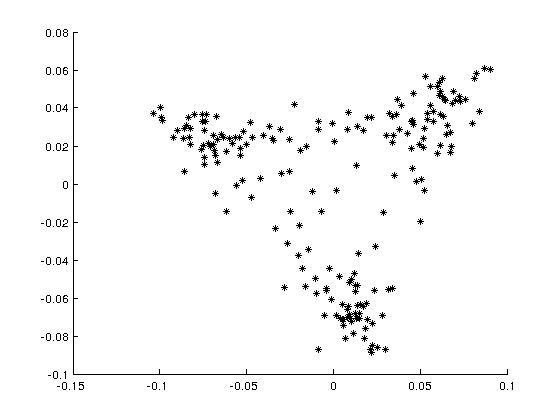
\includegraphics[width=0.35\textwidth]{c1.jpg}
        }
        \subfigure[Algorithm illustration with $\delta=0.8$]{

           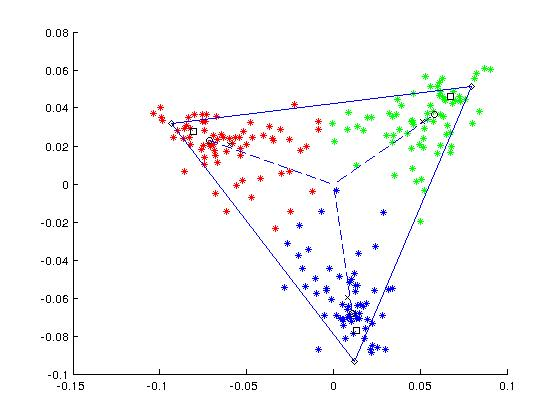
\includegraphics[width=0.35\textwidth]{c2.jpg}
        }\\ 
        \subfigure[$\alpha=0.8,\beta=0.25,k=3$]{

            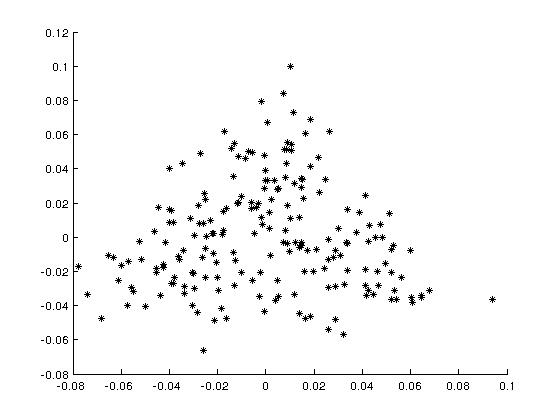
\includegraphics[width=0.35\textwidth]{b1.jpg}
        }
        \subfigure[Algorithm illustration with $\delta=0.8$]{

            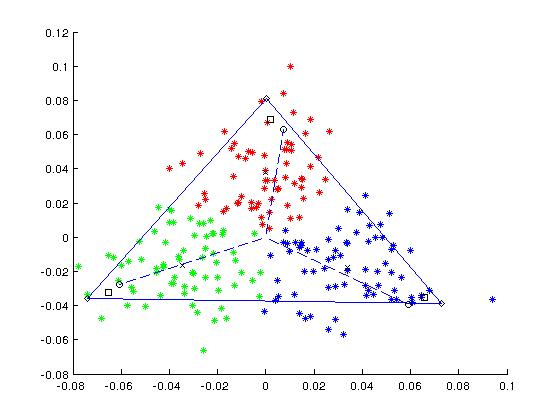
\includegraphics[width=0.35\textwidth]{b2.jpg}
        }

    \end{center}
{\small
    \caption{Illustration of Projector. The left figures are the $V_i$'s after the SVD step. In the right figures, the black 'o's at the ends of dotted lines are the real topic, black $\times$ are the $C_i$'s before scaling, black $\diamond$ are $C_i$'s after scaling, and black $\Box$ are the recovered $\hat{A}_i$'s. All points in the plot are after shifting and projected on the SVD subspace. }
}
   \label{fig:subfigures}
\end{figure}


We use estimated $\hat{A}$ and the inference procedure of the LDA
algorithm to predict words for testing documents. We use the inference
procedure of LDA since LDAT also uses it, and then we can attribute
the performance difference between LDAT and Projector to the quality
of $\hat{A}$ compared to the real topics.

We also experimented with a version of projector which does
not use LSI as a first step; it just proceeds
with $k$-means, then we project the documents into the subspace
that contains the means and scale as above.  The results
were quite similar to the results above so we do not
include them here. 

%% \subsection{Projector with $k$-means}

%% We run 
